\chapter{Modeling \& Specification}

% the spin reference manual will be useful for this part

The first two steps in model checking is to translate the sought design into models that can be understood by the model checker and defining the properties specified on the system. This chapter covers the process of these two steps, by first defining some building blocks used and then describing the final models.

%The modeling will first be described 

\section{Definitions}

First we will explain how a typical design, for a \wsn we seek to model, looks. Secondly we will describe in detail how each entity, referred to as \textit{Actors}, operates. Finally, before explaining the modeling, we will explain the meaning of some key aspects of the work such as \textit{Decisions} and \textit{Over-Collection}.

\subsection{Basic WSN}

A basic \wsn was defined as a starting point for the models. It consisted of a set of collection nodes (referred to as "nodes"), a central server (referred to as "Server") and finally an Environment (the observed source). An illustration of this can be seen in Figure~\ref{fig:basic_wsn}. Which is the basis for all the models described in the thesis. An important note on this setup is that the "environment" here is considered an entity (same as a node or a server). This abstraction was made to simplify the modeling, so the nodes instead of managing a shared resource instead can have the data communicated to them as messages.

\begin{figure}[ht]
    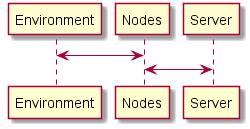
\includegraphics{include/figures/basic_wsn}
    \caption{An illustration of a \wsn}
    \label{fig:basic_wsn}
\end{figure}

%As a start for the formal development process, the project required some "building blocks" \todo{find a better word} to better define certain aspects of a \wsnd. 

%We will henceforth refer to entities in the system as \textbf{actors} in the system.

\subsection{Description of the Actors}

% describe a general network

A \wsn is built up by several different entities that communicates data between each other. Generally a network consists of multiples of virtually the same entity, e.g. multiple collection nodes, where each of these are running the different instances of the same process. Throughout the thesis these entities will be referred to as \textit{Actors}.\todo{motivate why?}

To describe the interaction between two actors in the system, behavior models were used (e.g. Figure~\ref{fig:behav_example}). Where the name of each actor is shown in the boxes at the top. The message channel used between them is shown as the arrows, where the arrow-head points to the actor receiving the message and the contents of the message is referenced above it. Finally the ordering of the messages are in a ascending order from the top, meaning the first message sent is shown furthest to the top of the figure.

% describe why the environment is modeled as such
% describe that the environment came later of directly?

% explain how i use them

\subsection{Over-Collection}

%A \wsn primary objective is to collect data from an observed source and let a processing unit analyze the state of it. 

In the paper \textit{insert reference to chapter 2 here}, they defined \textit{Data Over-Collection} to be "Collecting data more than enough on original function while within the permission scope". 

%For this to be true, we make the assumption that it exists a state for the system where the process of collecting data isn't required for the system to function the way it's intended. This could arise from a number of origins, either that a threshold has been reached and the system is no longer stable or that 


%Consider a collection process collecting some personal data from a users. The process is only interested in collecting as much data as possible and storing it at a central server for future processing. We can assume that the process will need a good quantity of data entries to extract relevant information from the data. If we assume that the program doesn't remove any data it's collected, we can safely say that at some point the system will have collected enough data to accomplish the tasks it's designed to do and beyond that point it's collected more than it requires.

% describe what over-collection means
%With a collection-process 'mindlessly' collecting personal data and storing it, we can assume that there's state where the collection has collected more data than it requires to complete whatever function the system is designed to do. 

\begin{definition}{def:Coll}{}
(Collecting)

A process $P$ collects a data point $d$ in a state $s$ if after leaving the state then $d \in \{P_{c'} \setminus P_{c}\}$.

%A process $P$ collects a data point $d$ in a state $s$ if after leaving state $s$ ($s_{+1}$) then $d \in P.lvars$\todo{promela syntax for local variables, should be something else}.
\end{definition}

\begin{definition}{def:ToFunc}{}
(To Function)

\textit{if a process P yields a valid result by a specific amount of input parameters, we say it requires these input parameters}
\end{definition}

% shall i really include time as a variable in my definition? snapshots seems better.
% We can consider two possibilities of systems, one where the system doesn't remove data from it's collection on it's own and one where it removes data over time.

\begin{definition}{def:OverColl}{} 
(Over-Collection)

\textit{if a process P collects more data than it "requires to function", we say a process is over-collecting.}
\end{definition} 

%\textbf{Formal Definition: } 
%Let a process P be able to collect data entries and to evaluate boolean expressions. 

%$P_{collect}: D \cup P_{collection}$

%where $P_{collection}$ means the set of data entries $(D_1,D_2,\ldots)$ collected, intially $\emptyset$, and $D$ is a new data entry being collected.

%$P_{eval}: D \rightarrow \textbf{Bool}$

%Let a service $S(x, y, ...)$ be a boolean expression depending on variables $x, y, ...$ 

%We say the process $P$ dedicated to the service $S$, noted $<P,S>$, over-collects data if and only if $P$ collects any data concerning one of the variables appearing in $S$ after $S$ has been evaluated to be true.

%$<P,S>$ over-collects iff $ \{ D \in P_{collection} \} \wedge \{ P_{eval}(D) = \textbf{True}\}$ \todo{something like that, but with S}

%$P = (C,E)$ $C$ is a finite set where the elements are tuples of $c \in C : c = (x,y,...)$ called data entries. $E: c \in C \rightarrow \textbf{Bool}$ (E is a function on an element in C with a resulting boolean value.) if $\left\{ { E: \exists c \in C \rightarrow \textbf{True} } \right\} \wedge \left\{ { S(x,y,...) \rightarrow \textbf{True} } \right\}$ and $c = (x,y,...)$ (translation between variables and c).

%Let $\textbf{D}_C$ be a new data point not in the collection and $\textbf{D}$ be the current stored collection of data. Let $|D|$ be the amount of data entries in $\textbf{D}$ and $\textbf{F}$ be a fixed number describing the amount of data a process requires to function.  

%So consider a system that is not in a over-collective state ($|\textbf{D}| < \textbf{F}$) is receiving a new entry point to it's collection; 

%\[ \textbf{D} + \textbf{D}_C = \textbf{D}' \]

%Where '+' means the operation of appending the data to the collection. So then if:

%\[ |\textbf{D}'| \geq \textbf{F} \]

%Then a system is over-collecting.

% assume non-dissipating? personal data not being removed?

% formal formulation (like non-inference)

%*overcollection-examples*

%*define over-collection*


\subsection{Decisions}

%introduction leading up to what we need it for.

A \textit{decision procedure} is an algorithm that terminates with a yes or no answer, given a decision problem.\cite{decisionproceduresbook} 

%From the Definition~\ref{def:OverColl} we understand it's not uncommon for processes to collect more data than they require. 

% A single sensor node usually\cite{WSN_a_survey} doesn't hold enough information about the system state to 


%\subsubsection{Formal Definition}

%\begin{definition}{}{}
%\label{def:DecProc}
%(Decision Process)

%A process is called a decision process for T if it is sound and complete with respect to every formula of T.
%\end{definition}

%\textit{Definition \ref{def:DecProc} also requires some more definitions, but this is an important one so added it for now.}

%\begin{definition}{}{}
%\label{def:DecComplete}
%(Completeness of a procedure)

%A procedure for the decision problem is complete if 
%\begin{itemize}
%\item it always terminates (termination), and
%\item it returns "Valid" when the input is valid. (soundness)
%\end{itemize}

%\end{definition}


%A decision \todo{rewrite} is a control message sent through the network forcing an action to be taken\todo{witness? semantics?}, in this report that's mainly when over-collection is occurring. This can for example mean that the server is telling one (or several) collection nodes that they should shut down or wait until sending again. If the nodes are also computing data they can still be kept doing so but without sending communication throughout the network until notified again. The source of the decision depends on if the network has a centralized processing unit (f.e. a master-slave relation) or if computations are decentralized and each processing unit makes decision on their own and uses communication to forward processed data to a storage server. 

%\textbf{Definition: } A message sent in the network is considered a decision if it changes the behavior of an actor.

%*formally define decisions* ?


\section{Modeling}

%*what is a model?*

As a starting point for defining the models, first different architectural choices were considered. This was done to help define different cases of \wsn that could use decisions. 

\subsection{Variations}

The different variations considered were: \\

\begin{itemize}
\item Centralized or Decentralized decision making
\item Conjunctive or Disjunctive decision analysis
\item Centralized or Distributed communication
\end{itemize}

\subsubsection{Decision Making}

The first choice reflected how much the sensor nodes would analyze the data. Since nodes can have a processing unit, they could potentially analyze the collected data and make a decision on their own. 

\subsubsection{Decision Analysis}
The second choice reflected how the decision were processed, if the data from a single data point could trigger a decision or if the decision considered data from multiple entries in it's evaluation.

\subsubsection{Communication}

The final variation reflected how the network communicated, it was considered centralized if all communication were sent through a central unit, such as a server, or if nodes were allowed to communicate independently to each other.

\subsection{Initialization}

An initial model was made for one variation, a model with a centralized decision making, disjunctive decision analysis and centralized communication. This was made as a starting point for other variations and also help define the properties sought of the network.


%This was due to that this variation appeared to be the easiest to implement and analyze, which in turn would help making the other variations and as well formalize the properties sought of the network.

Furthermore, the project defined the individual components of the \wsn to three actors: \textit{Node}, \textit{Server} and \textit{Environment}.

%Furthermore, the project sought to define a model for the basic \wsn \todo{from 2.1 ref?}, so three actors were defined: \textit{Node}, \textit{Server} and \textit{Environment}.

%Initial models were made for each of the choices except conjunctive decision procedures. 

%This was due to that a conjunctive decision procedure would require a more sophisticated algorithm to analyze the data than the other choices, which would require additional time for just one variation. \todo{is this a relevant chapter?} 

%As suggested when developing formally, I started out with a simple model \todo{only explain how I started out in intro / conclusion} as possible. So the model expects that each actor acts as intended, without malicious users or failing procedures, and that all messages gets through, e.g. no 'lossy' channels. 

%Furthermore, the project sought to define a model for the basic \wsn \todo{from 2.1 ref?}, so three actors were defined: \textit{Node}, \textit{Server} and \textit{Environment}.

\subsection{Server Actor}

The server is an actor receiving messages from nodes and storing it for later usage. A server's behavior will vary depending on the structure of the system. If the decision is taken centrally the server will be the one checking for over-collection, otherwise it will be a node. Also if the communication is managed through the server, if the nodes doesn't communicate with each other, the server will act as a repeater for the decision. 

\begin{figure}[ht]
    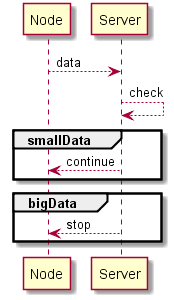
\includegraphics{include/figures/server_behav}
    \caption{Behavior Model between Server and the Node}
    \label{fig:node_server_behav}
\end{figure}

In Figure \ref{fig:node_server_behav} is the behavior for a system where server makes the decision and nodes doesn't communicate with each other. First, the node sends some data, the server checks for over-collection and replies accordingly. The response will either be a "stop" signaling that over-collection has occurred and the node should stop collecting or it tells it that it can continue collecting. 

In addition to the behavior model, an Finite State Automaton(FSA) were designed for the server (Figure~\ref{fig:server_states}). The initial state being \texttt{Idle\_a}, which the server will stay in until some \texttt{data} is received. "Data" being either \texttt{bigData} or \texttt{smallData}; $ \texttt{data} \in \{ \texttt{smallData}, \texttt{bigData} \} $. The data is received in \texttt{Idle\_a} and \texttt{Idle\_s} and then checked in \texttt{Answ.} and \texttt{Hold}, meaning only the outgoing transitions from \texttt{Idle\_a} and \texttt{Idle\_s} is incoming data, the other are calculated internally. This also means the server will loop indefinetly between \texttt{Answ} and \texttt{Idle\_a} as long as only smallData is received. When \texttt{bigData} is received the server will enter the \texttt{Idle\_s}-\texttt{Hold} loop instead, which denotes the states where the server is requesting the nodes to stop collecting more data. 

%This behavior can be described using states as well, as shown in Figure \ref{fig:server_states}. The same notations are used for the messages sent between the actors except "check" is noted as the state named "Waiting".

\begin{figure}[ht]
    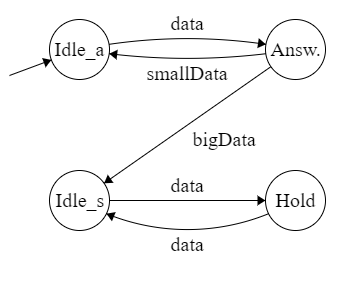
\includegraphics{include/figures/server_actor_fsm}
    \caption{Finite State Automata for the Server Actor}
    \label{fig:server_states}
\end{figure}

\subsection{Environment Actor}

The process for the environment actor had two steps:

\begin{enumerate}
\item Generate random data
\item Serve random data to a requesting node 
\end{enumerate}

As mentioned before, the first step is not intuitive for an environment since the observed source isn't randomly varying, but for modeling purposes this is a simplification made to reduce the complexity of the model. In Figure \ref{fig:behav_example} the behavior between a node and the the environment is described.

%Each node requesting data is placed in a FIFO-queue to the environment, meaning the environment will serve the node that's waited the longest during each iteration. 

\begin{figure}[ht]
    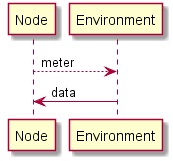
\includegraphics[]{include/figures/env_behav}
    \caption{Behavior Model for the Environment}
    \label{fig:behav_example}
\end{figure}

The corresponding FSA for the environment is seen in Figure~\ref{fig:env_states}. The environment will stay in the initial state \texttt{W} (short for "Waiting"), until a node \texttt{meter} it. Then the data is "generated" in \texttt{G} (short for "generate data") and served back to the node.  

%This behavior can be described using states, as shown in Figure \ref{fig:env_states}. Here the process starts in a waiting state and when a node meters it, some data is generated and sent to the node.

\begin{figure}
    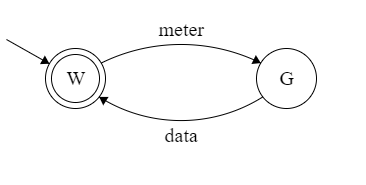
\includegraphics{include/figures/environment_actor}
    \caption{FSA for the Environment Actor}
    \label{fig:env_states}
\end{figure}

\subsection{Node Actor}

As seen in the behavior model for the node actor (Figure \ref{fig:node_behav_smallData}), it captures the majority of a typical scenario for the entire system. That is intuitive since the node communicates with both of the other actors of the system and is a intermediate\todo{is this the right word?} part of the system. The scenario is when a node collects data, that doesn't cause a system-change, and forwards it to the server.

\begin{figure}[ht]
    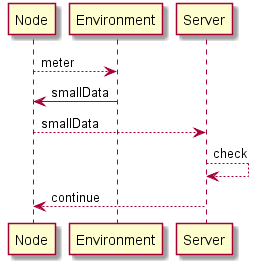
\includegraphics[scale=1]{include/figures/node_behav_smallData}
    \caption{Behavior Model for a Node}
    \label{fig:node_behav_smallData}
\end{figure}

The alternative behavior for system is described in Figure \ref{fig:node_behav_bigData} instead. There the data collected causes the server to make the decision that the node should stop collecting.

\begin{figure}[ht]
    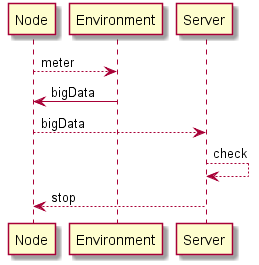
\includegraphics[scale=1]{include/figures/node_behav_bigData}
    \caption{Behavior Model for a Node over-collecting}
    \label{fig:node_behav_bigData}
\end{figure}

This behavior can be described in a FSA, as seen in Figure~\ref{fig:node_states}.\todo{argue why I've kept the states to a minimum here?} The node meters data from the environment and passes it forward to the system. There it waits (noted by the state \texttt{Wait}) for a response before returning to the \texttt{Idle} state.

\begin{figure}[ht]
    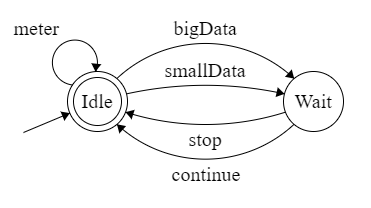
\includegraphics{include/figures/node_actor_fsm}
    \caption{FSA for the Node Actor}
    \label{fig:node_states}
\end{figure}



%The environment is a simple procedure, it starts off by generating random data and serving it to a requesting node. This is a modeling simplification, since the node should rather extract the data from the environment rather then be waiting for a response. But this was made to simplify the system and made the environment easier to manage as a shared resource for the nodes. 

%The collection nodes follows the same procedure, where they start by 'requesting' data from the environment. Then the model was split into two different choices depending on the structure of the system. If the system was decentralized, the decision could be taken by a node. Meaning that then the node would first check if the data requested from the environment was below a certain threshold. Then it would send the data along to the server with either a message 'go', meaning that all was fine, or a message 'stop' meaning that over-collection was occurring and it was going to stop collecting and the other nodes should do the same. 

%If the system was a centralized one, the node would simply pass the data forward to the server. Then it would wait for a response to see if it should continue collecting or if it should stop. This describes a typical scenario for the system, so from this a behavior model for each actor can be defined.

%\[ image here \]

%The behavior model of the nodes can explain the behavior of the entire centralized system, since the node 'communicates' with all the involved parts and is the one taking (being effected of) all the actions. What distinguishes the decentralized system and the centralized can be noticed in the behavior model for the nodes, in the state marked 'data retrieved'. Here the node would check the data on it's own and notify the server of the action being taken, but the behavior model still works for both cases.

%This model expects a perfect behavior from all actors involved, since it doesn't take into account bad behavior (e.g. message-loss or malicious usage) which is not unlikely to occur in a WSN. But this isn't meant to be captured by the model either at this stage, but will be considered when later extending the model.  

%*explain what this model doesn't consider and possible variations for the decisions.*
\newpage
\section{Specification}

This section presents the properties used to verify the system. The process of defining the properties were an iterative approach and several versions were considered, this section only covers the final properties were the result of this process. 

\subsection{Properties}

The properties defined on the network were formulated using \textit{Linear Time Logic} (LTL). This choice came from the fact that LTL were native to SPIN and the models were abstracted to only focus on the relevant parts to the project, LTL could provide a simple and direct specification to that problem.

\subsubsection{Correctness}

The primary property sought of the system was that it was working as intended. This was formulated as a safety correctness property, to ensure that when decision had been taken, the system respond to the by changing its' behavior.

% explain correctness some more

\begin{definition}{}{} 
Safety Correctness

\textit{When the stop-decision is taken, the system should stop collecting.} \\ 

LTL: $\Box (O \rightarrow (\Diamond D)) $ \\
\end{definition}

Where \textbf{O} and \textbf{D} corresponds to the state where the stop-decision is taken and the states where collection is stopped respectively. This captures the sought system change; whenever the system reaches the state O, eventually it will reach state D. An immediate change is not required, therefore the timing\todo{is this the proper word?} is relaxed by the eventually-operator.

\subsubsection{Liveness}

%A liveness property should express that "eventually something good happens" which for this project became that "eventually a node communicates data to the server". This didn't entirely capture what was sought from the system so an additional property was added for "if a data is communicated to the server, eventually the server replies to the node". 

The second property was intuitive for the system since the initial models were constructed in such a way that when data is sent to the server, the first thing the server does it analyze it and respond accordingly depending on what data was sent.\todo{mention it was verified by design?}  

\begin{definition}{}{}
Liveness (sending)

\textit{Eventually a node sends it's data to the server.} \\

LTL: $\Diamond$ Node\_Send \\

Where Node\_Send denotes the state where the node sends the data to the server. \\
\end{definition} 

\begin{definition}{}{}
Liveness (replying)

\textit{If a node sends data to the server, eventually the server replies to the node.} \\

LTL: $\Box ($Node\_Send $\rightarrow \Diamond$ Server\_Reply$)$\todo{server\_reply doesnt exist atm.} \\

Where Node\_Send means the same as previously and Server\_Reply denotes the state where the server responds to the node.
\end{definition}

%Where \textbf{D} and \textbf{O} are the same events as described previously.